%-----------------------------------------------------------------------
\section{Methodology}
%-----------------------------------------------------------------------
%\tbc


This section gives some information on how to proceed to achieve the  objectives described in section \ref{sec:Objectives}.
As decided previously in the project, the means chosen to design the WP3 software, compliant to SIL4 requirements of EN50128 are SysML on Papyrus and SCADE for the modelling part, C language for the executive software. The first versions of the OpenETCS toolchain already involve Papyrus.

Other tools can be involved to support the task of the workpackage (indeed to manage requirements, data, traceability,...) but will be defined latter depending of the needs and the propositions.

For further information on means selection and detailed description of the process, consider the deliverables [D7.1]\footnote{\url{https://github.com/openETCS/toolchain/blob/master/T7.1/D7.1/D7.1.pdf}}, [D7.2]\footnote{\url{https://github.com/openETCS/toolchain/blob/master/T7.2/D7.2/D7_2.pdf}} and [D2.4]\footnote{\url{https://github.com/openETCS/requirements/blob/master/D2.4/D2_4.pdf}}.

\subsection{Main step of the analysis}

The figure \ref{fig:Steps} gives the main steps of the design approach and main used and produced artefacts. All is detailed in D2.4.

\begin{figure}[ht]
  \centering
  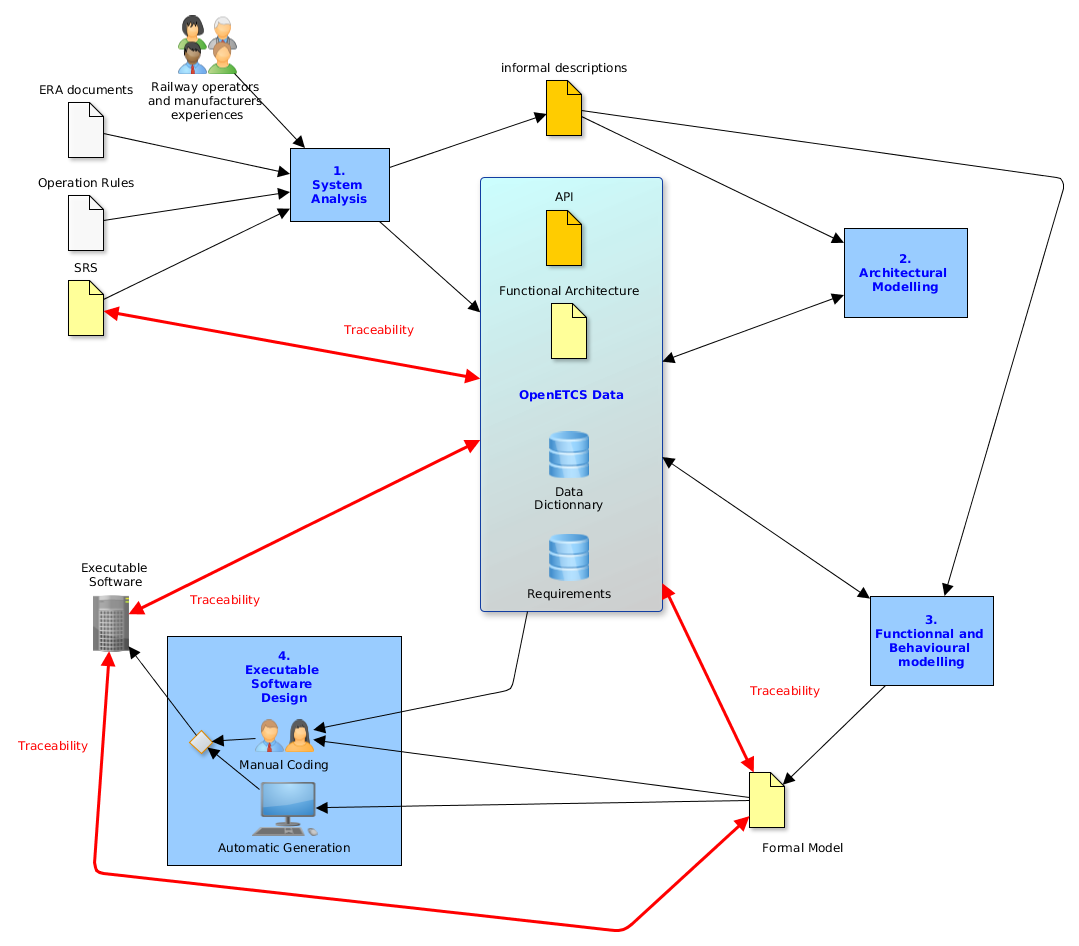
\includegraphics[width=\textwidth]{sections/Step.png}
  \caption{Main steps of the design approach}
  \label{fig:Steps}
\end{figure}


Four main steps are defined:
\begin{description}
\item [System Analysis] to identify the main functions and their interactions and to clarify the requirements allocated to them.
\item [Architectural Modelling] to specify the functional architecture of the system to design and internal and external interfaces. In parallel  the main data exchanged between the functions shall be identified.
\item [Functional and Behavioural Modelling] to provide a formal model of each function.
\item [Executable Software Design] to provide executable part of software.
\end{description}

These steps are sharing common artifacts which going to be updated and completed during all the design phase. Some recommendations and guidelines are defined in D2.4 for naming of elements or specifing a model.

As the artifacts are shared, an iterative process can be easily applied at each level.

\subsection{Shared artifacts}

\subsubsection{Functional architecture and API}

API\footnote{\url{https://github.com/openETCS/requirements/blob/master/D2.7-Technical_Appendix/OETCS_API\ Requirements_v1.0Draft_130301.pdf}} is a document provided as input which can be updated according to the needs.

Functional architecture is specified as a SysML  model, which can be automatically translated in a Scade model. An initial SysML model to cover the initial functional scope \ref{sec:FunctionalScopeTheMinimumOBUKernelFunction} is available on github: \url{https://github.com/openETCS/modeling/tree/master/model/sysml}

See D2.4 for how to use SysML to define the Functional Architecture.

\subsubsection{Set of Requirements}

The initial  set of requirements is the contains of Subset\_026 v3.3.0. These requirements are available as ReqIF format on github: \url{https://github.com/openETCS/modeling/tree/master/model/subset26}
.

This set is going to be increased during the design with updated requirements and added requirements.

Data model of D2.4 gives the information to manage on the requirements.

For the moment, ProR is involved in the openETCS toolchain to define new requirements and links between them.
It is still to clarify how to manage traceability.



\subsubsection{Data Dictionary}

The Data Dictionary is the set of all the types, constants and variables defined to  describe the system.
Data model of D2.4 describes how to define a data.

A preliminary task of the system analysis is to identified and specify the data structure which allow to describe the system.

Then the data structure and data definition shall be implemented in the data dictionary.

For the moment the mean to do this implementation is not clearly identified (UML library ? XML files ?)


\subsubsection{Formal models}

Two  models are provided during this phase:
\begin{itemize}
\item  a semi-formal model in SysML which gives the functional architecture of the system, including interaction between each function  and definition of the data.
\item a formal model in SCADE which follows and completes the same architecture and gives a behavioural description of each function. Then C code can be automatically  generated from this model.
\end{itemize}

\subsection{Function specification and design}


For the specification and the design of a functional block, a set of subtasks can be defined:

\begin{enumerate}
\item Identify the function and the input document to describe it (requirements of subset 26 or other subsets, API,, functional architecture,...)
\item Specify its environment and its external interfaces with an ibd diagram in SysML
\item Define and specify  its internal decomposition in subfunctions and its internal  interfaces with ibd and bdd diagrams in SysML
\item Link and complete to the data dictionary
\item Allocate and manage the requirements
\item Clarify and specify the behavior of each elementary function in SCADE
\item Complete Data dictionary if necessary
\item Complete requirement sets and manage traceability
\item Provide for review
\end{enumerate}